\chapter{Stellar Activity Modelling in Radial Velocity Time Series}
As discussed in Sect.~\ref{sect:activity}, there exists a multitude of physical
processes ongoing within the photospheres and chromospheres of active stars
which produce observable signatures with a variety of amplitudes and timescales
(see Table~\ref{table:activity}). The subsequent sections discuss a variety of
techniques which have been used to model and consequently mitigate the effects of
stellar activity in RV time series.

\section{An Overview of Techniques for Stellar Activity Mitigation}
\label{sect:methods}

\subsection{Stellar Activity as a Scalar Parameter}
Back when the first giant exoplanets where being discovered with RVs,
typically a treatment of stellar activity was not implemented. The reason being
that the quality of the datasets at that time were insufficient to resolve the
temporal structure of RV activity for any but the most active stars. Many
observers however did report the root-mean-square (rms) of their RV residuals
following the removal of their best-fit planet model
\citep[e.g.][]{mayor95,butler96}. In
many cases this revealed residaul rms values which exceeded the characteristic RV
measurement uncertainty and thus alluded to the presence of additional
jitter signals which may or may not vary significantly with time. \\

In many of the following RV planet searches the apparent jitter was characterized
by an additive scalar $s$. The free parameter $s$ was used to characterize the
level of RV jitter as it was added in quadrature to the RV measurement
uncertainties when evaluating the objective function during any analysis
equivalent or analogous to a $\chi^2$-minimization routine. The nature of this
method assumes a fixed level of dispersion due to jitter that is constant in time.
As such, the resulting
measurement of $s$ does little more than inform us of the jitter amplitude as
any temporal evolution of activity, due to finite active region lifetimes or magnetic
cycles, will remain unresolved.

\subsection{Correlations with Activity Indicators}
Stellar RV observations are known to be affected by both planetary companions as
well as by stellar activity. Disentangling those signals in RV time series
therefore benefits significantly from ancillary time series which are sensitive
to stellar activity only \citep{boisse09}.
The classical implementation of de-correlation by
an activity indicator is to derive time series of one or many spectroscopic
activity indicators whose sampling is simultaneous with the RVs and then
fitting an often linear relation between those datasets (Fig.~\ref{fig:corr}) to
account for the temporal evolution of activity over the observational baseline.
The relation, when fitted simultaneously with planetary solutions, allows the RVs
to be de-correlated jointly with the measurement of the planetary parameters.
This technique has been shown to be effective when the stellar rotation period
\prot{} is well constrained, the planetary orbital period is distinct from
\prot{,} the amplitude of the planetary signal exceeds that of the activity signal
by $\gtrsim 30$\%, and the stellar rotation period is well sampled over multiple
cycles \citep{boisse11}. \\

\begin{figure}
  \centering
  %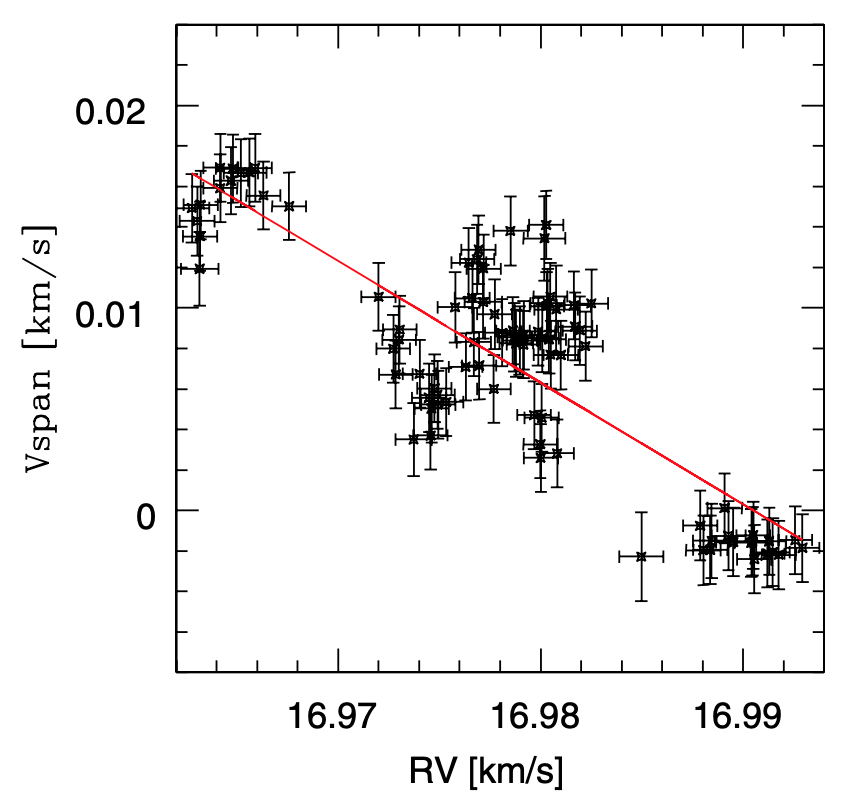
\includegraphics[width=.6\textwidth]{figures/vspan_rv.png}
  \caption[Correlation between stellar RVs and the \vspan{} activity indicator.]
      {The correlation of the \vspan{} activity indicator with the RVs for the
    active Sun-like star HD 17051 from HARPS spectra. The solid line depicts the
    best-fit linear relation from least squares fitting. The fitted relation is
    used to de-correlate the RVs for the effects of stellar activity as probed by
    the \vspan{} time series. \citep[Image credit:][]{boisse11}.}
  \label{fig:corr}
\end{figure}

There exists a number of activity indicators which can be derived from the stellar
spectra. There definitions and physical motivations are summarized below. \\

\emph{log R$'_{HK}$}:
the \caii{} H and K resonance lines are excited by non-thermal heating 
and act as a sensitive indicator of chromospheric structure and particularly of
the presence of bright chromospheric plages. 
For optical spectra with access to the \caii{} H and K lines
centered on 3968.47 \AA{} and 3933.66 \AA{,} the Mt. Wilson S-index is defined as

\begin{equation}
  \text{S-index} \propto \frac{\Psi_H + \Psi_K}{\Psi_B + \Psi_V}
\end{equation}

\noindent where $\Psi_H$ and $\Psi_K$ represent the narrowband
($\sim 1.1$ \AA{} wide) fluxes in the cores of the H and K lines of the \caii{}
doublet. The index is normalized by total flux in the $B$ and $V$ continuum bands
which are 20 \AA{} wide broad bands centered on 3900 and 4000 \AA{} respectively.
From this the \Rhk{} indicator is derived using a variety of formulations which are
all $\propto$ S-index and attempt to isolate the chromospheric component of
$\Psi_H$ and $\Psi_K$ from the photospheric component using normalization factors
which are dependent on \teff{} and level of stellar activity \citep{lovis11}. The
\Rhk{} indicator has been well characterized as a sensitive probe of activity on
both Sun-like stars and M dwarfs
\citep[e.g.][]{wright04,lovis11,astudillodefru17b}. \\

$H\alpha$: 
similarly to the \Rhk{} index, H$\alpha$ photons ($\lambda = 6562.81$ \AA{)} are emitted by
hot plages and thus act as a tracer of stellar activity originating from the chromosphere.
H$\alpha$ may act as a more suitable spectroscopic activity indicator for cool M dwarfs
which of lack significant flux in the \caii{} H and K lines \citep{robertson14}.
In practical terms,  
similar spectral features tracing a star's chromospheric structure may alternatively be used
as activity indicators depending on the accessible wavelengths of the employed spectrograph
(e.g. \hei{,} \nai{,} etc). \\


\emph{CCF shape parameters}:
the cross-correlation function (CCF) of a stellar spectrum represents its average line profile
at typically a high S/N.
As illustrated in Fig.~\ref{fig:starspot}, the presence of active regions distorts
the Gaussianity of the CCF thus alluding to the presence and nature of those active regions.
A number of shape parameters to the fitted CCF may be used to characterize stellar activity
using the same CCF from which the stellar RVs themselves are derived. However, these
spectroscopic diagnostics are only useful when they are robustly derived from high S/N
spectra of active stars where their effects on the CCF are clearly discernable \citep{desort07}.
Examples of three
shape parameters are visualized in Fig.~\ref{fig:ccf} and described below. \\

\begin{figure}
  \centering
  %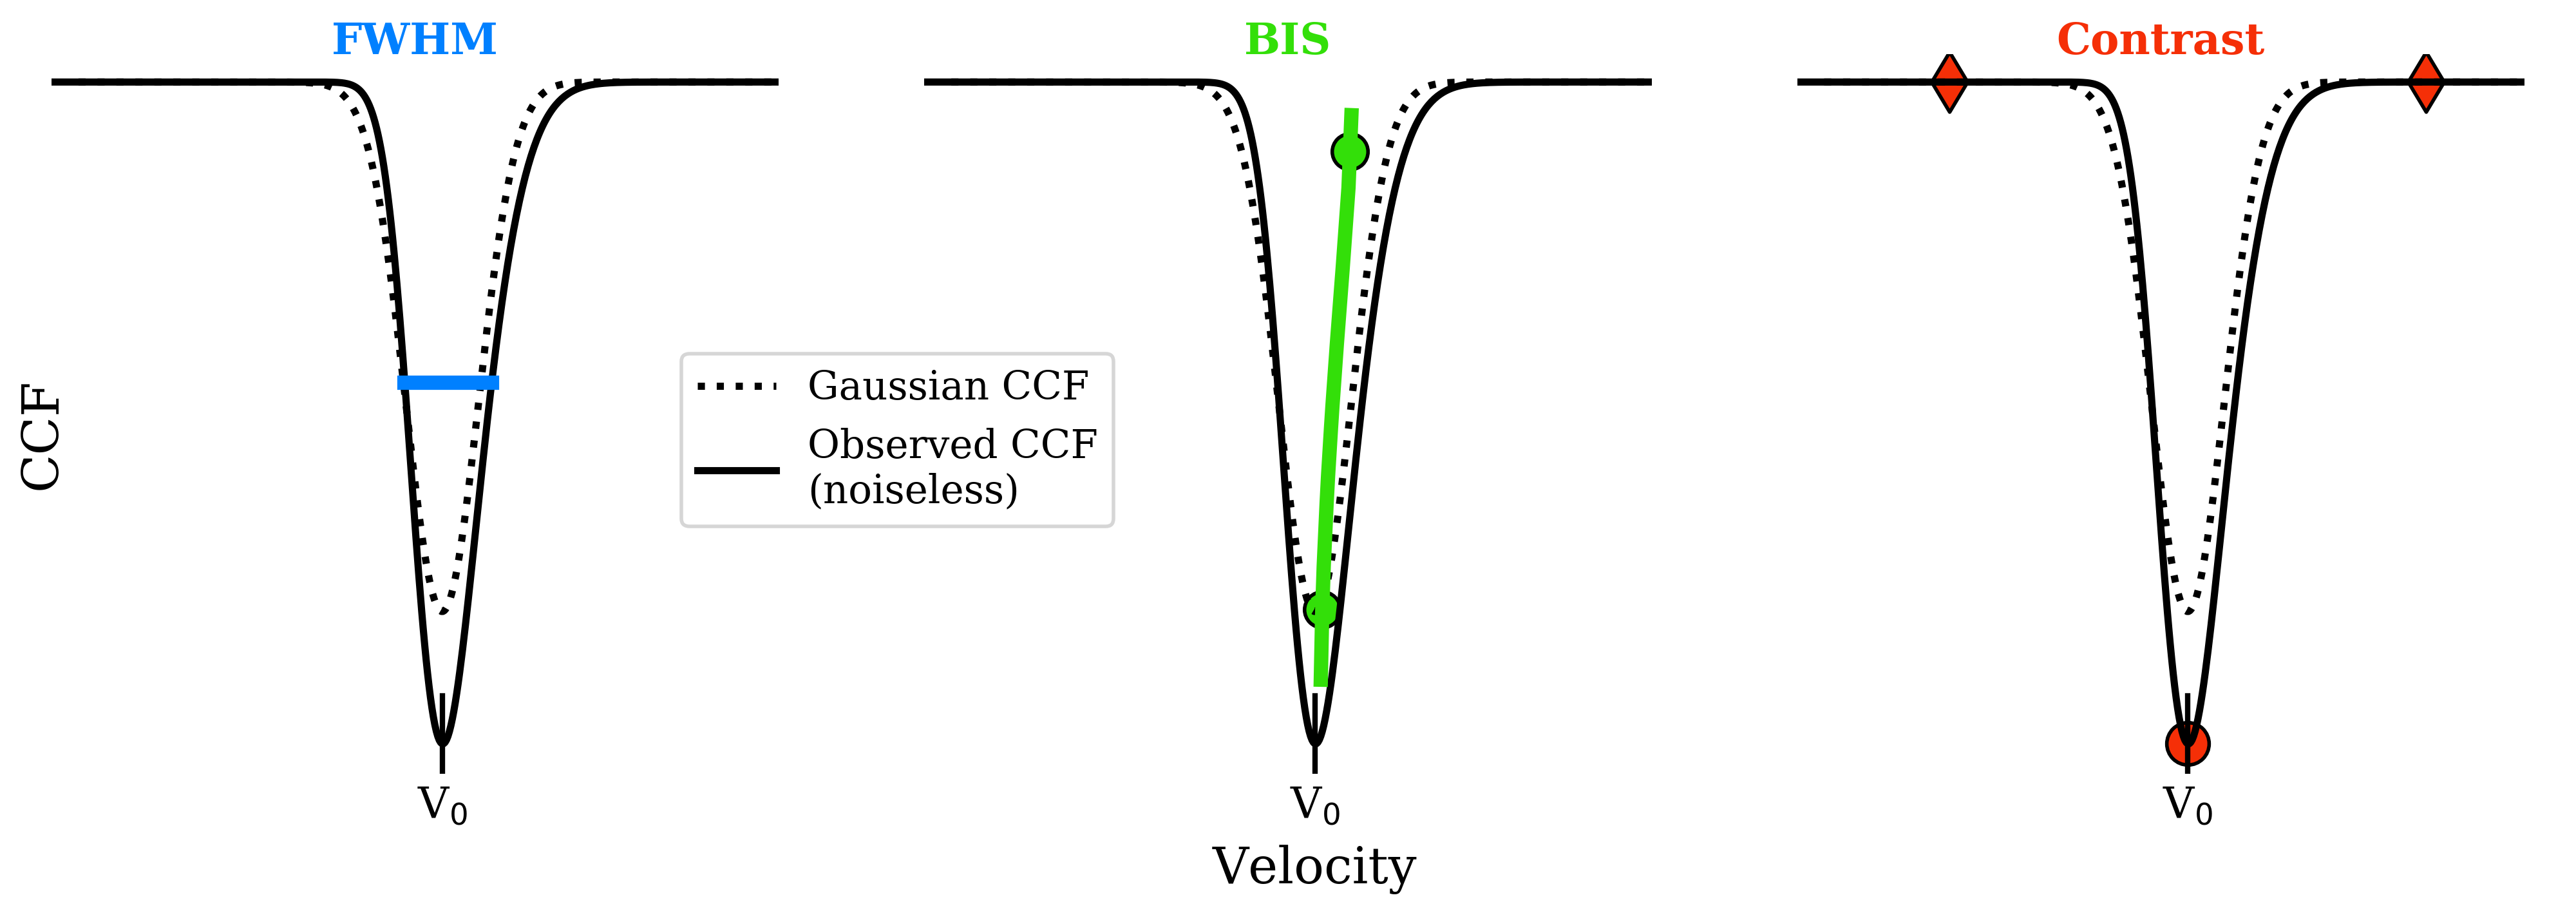
\includegraphics[width=\hsize]{figures/ccf.png}
  \caption[Illustrations of CCF shape parameters.]
          {Illustrations of measurements of the CCF width, asymmetry, and contrast via the full
            width half maximum (FWHM), bisector (BIS), and contrast shape parameters. The FWHM
            characterizes broadening of the CCF due to active regions at unique velocities on the
            stellar disk. The
            BIS characterizes the asymmetry of the line profile by computing the difference in
            average velocity in the upper and lower portions of the CCF (green circles in the
            middle panel). The contrast characterizes the depth of the CCF by taking the average
            of the CCF in the contiuum (diamonds) and its difference with the CCF flux at the
            stellar velocity $V_0$.}
  \label{fig:ccf}
\end{figure}

\emph{FWHM}:
the full width half maximum (FWHM) of the CCF is commonly used as a measure of CCF
width. As an active region transverses the rotating stellar disk across the differentially
Doppler-shifted limbs, its temperature contrast with the stellar photosphere adds additional
power to the CCF in the velocity direction opposite the occulted limb. This results in a
broadening of the CCF on one side of its mean velocity $V_0$. As illustrated in
the first panel in Fig.~\ref{fig:ccf},
the FWHM can be measured from the width of the CCF at a specified location. \\

\emph{BIS}:
recall that the broadening of the CCF due to a single active region is asymmetric about $V_0$.
A common shape parameter to characterize the resulting asymmetry is the bisector
\citep[BIS;][]{queloz01}.
Similar parameters have also been proposed as measures of CCF asymmetry such as the curvature of
the bisector line \citep{hatzes96}, the velocity span \citep{boisse11}, and the BIS inverse
slope \citep{queloz01}. Their definitions are closely related and rely on computing the weighted
velocity in the upper and lower portions of the CCF (see middle panel of Fig.~\ref{fig:ccf})
and computing their difference. A symmetric line profile will therefore have a BIS$=0$ whereas
asymmetric profiles affected by active regions will be non-zero and whose exact value and units
will depend on the defintion of the asymmetry parameter used. \\

\emph{Contrast}:
\citep{boisse09} noted that increasingly active stars, based on their fractional coverage by dark
star spots, tend to have shallower line profiles. This is the direct result of such stars featuring
greater contributions to their average line profiles from cool and therefore dimmer regions.
This effect is often characterized by the CCF contrast which is equal to the difference between the
average baseline of the CCF in the continuum (located many standard deviations away from $V_0$ in
the CCF wings) and the flux at the stellar velocity $V_0$.


\subsection{Photometric Modelling: the \textbf{\emph{FF}}$'$ Method} \label{sect:ffp}
An alternative to using simultaneous spectroscopic activity indiciators to temproally de-correlated
RV measurements for the effects of stellar activity, \citep{aigrain12} present the $FF'$ formalism
which uses contemporaneous photometry to model two distinct RV activity components. \cite{aigrain12}
argue that in the limit of small active regions with non-complex configurations, the fractional
coverage of the stellar disk by active regions (i.e. spots) $F(t)$ is related to the photometric flux
$\Psi(t)$ via

\begin{equation}
  \Psi(t) = 1 - F(t).
  \label{eq:ffp}
\end{equation}

\noindent Eq.~\ref{eq:ffp} reads that the fractional spot coverage is just one minus the observed
stellar flux in normalized units such that the star's brightness equals unity in the absence of spots.
The corresponding RV signals from a active regions giving rise to the photometric variations are known
as the rotation or flux effect $\Delta \text{RV}_{\text{rot}}$ and the convection blueshift effect
$\Delta \text{RV}_{\text{conv}}$. The former arises from active regions occulting the differentially
Doppler-shifted stellar limbs and thereby suppressing the flux of photons with a particular
Doppler-shift. Because the rotation effect affects the RVs in proportion to the spot coverage and
exhibits a sign change as the spot crosses from the blueshifted limb to the redshifted limb over a single
rotation cycle, the rotation effect is

\begin{equation}
  \Delta \text{RV}_{\text{rot}}(t) \propto F(t) \dot{F}(t)
\end{equation}

\indent where the first time derivative of the fractional active region coverage is
$\dot{F}(t) = -\dot{\Psi}(t)$ from Eq.~\ref{eq:ffp}. As such, the rotation effect tends to dominate
on rapidly rotating stars wherein $\dot{F}(t)$ is large. Conversely, the convective blueshift effect
operates by active regions disrupting the homogeneity of the stellar disk on which convective
blueshift is on-going everywhere. This disruption scales with the fractional spot coverage and
the angle between the spot normal and the line-of-sight which results in

\begin{equation}
  \Delta \text{RV}_{\text{conv}}(t) \propto F^2(t).
\end{equation}

\noindent The convective blueshift effect tends to dominate more slowly rotating spotted
stars such as the Sun \citep{haywood16}. \\

Fig.~\ref{fig:ffp} demonstrates both the rotation and
convective blueshift effects on the RVs and how they are related to the photometric detriment
incurred by a single spot over a portion of one stellar rotation cycle.

\begin{figure}
  \centering
  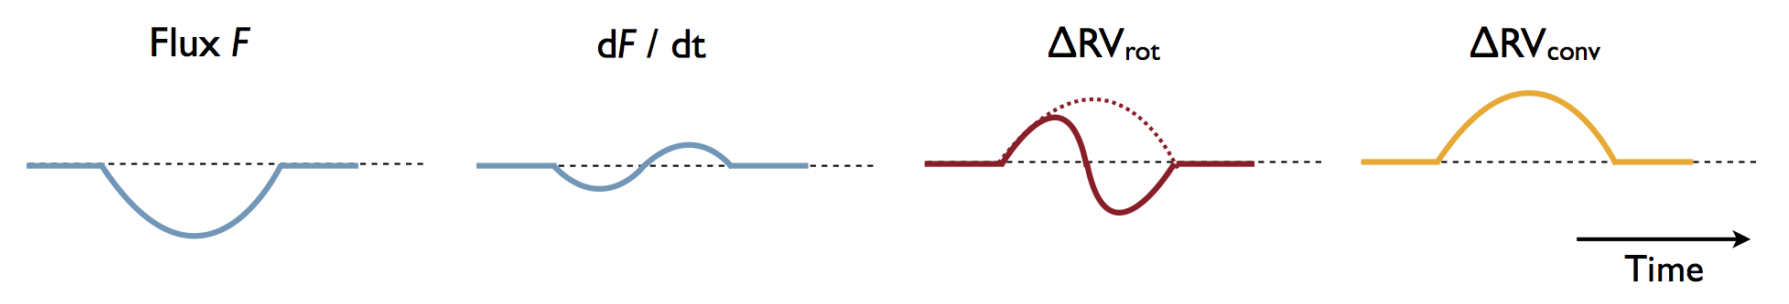
\includegraphics[width=0.8\hsize]{figures/ffp.png}
  \caption[Illustration of the $FF'$ method.]
      {The $FF'$ method for deriving the rotation and convective blueshift components
    of stellar RV activity from contemporaneous photometry. Here the photometric stellar flux
    is used to infer the fractional spot coverage $F(t)$. The rotation effect scales with
    $F(t) \dot{F}(t)$ and thus varies with half the period as does the convective blueshift
    effect which scales as $F^2(t)$. \citep[Image credit:][]{haywood15}.}
  \label{fig:ffp}
\end{figure}


\subsection{Pre-whitening}
This method aims at identifying strong periodicities in the RV time series and removing also
such signals until only residual Gaussian noise is remaining. This method known as pre-whitening
is based on analyzes of multi-periodic stellar oscillation modes and works by performing a Fourier
transform of the data and removing sinusoidal functions from the raw data whose periods and
identified by the frequency analysis \citep{queloz09}. Pre-whitening assumes that all signals
are long-lived and sinusoidal which is not always applicable for the stellar activity signals
that it aims to mitigate. 

\subsection{Deterministic Model Fitting}
RV time series exhibiting strong coherent signals at either \prot{} or its first
harmonic\footnote{As can be the case for rapidly rotating spotted stars whose RV activity
  is dominated by the rotation effect (see Sect.~\ref{sect:ffp}).} may be well modelled by
a deterministic function in the form of a sinusoid at \prot{} or $P_{\text{rot}}/2$
\citep{boisse11}. In general, such models are incomplete because they neglect any temporal
evolution of active regions which vary in their sizes, temperatures, and spatial distributions
over adjacent rotation cycles \citep{giles17}. These nuances are not captured in a 
deterministic sinusoidal model although this methodology may still be applicable in time series
with short observational baselines or for stars with long-lived active region groups.


%\subsection{Physical Models of Active Regions}
%\citep{dumusque14}


%\subsection{Spectral Feature Decomposition}
\subsection{Line by line radial velocities}
Spectral lines are known to be affected differently by stellar activity due to their
sensitivities to pressure, temperature, embedded magnetic field strength, and fluid
velocity which are all affected by stellar activity \citep{davis17,wise18}. These
effects from stellar activity to spectral line shapes are distinct from Doppler-induced
line shifts which are identical to all lines. \cite{dumusque18} investigated
the prospect of deriving stellar RVs line by line. The resulting RVs derived from
individual lines were shown to be
consistent with the archival RVs derived from the HARPS data reduction software.
The derivation of RVs in this way is postulated to mitigate anomalous RV signals
from stellar activity if spectral features that are minimally affected by activity
are utilized. Intelligent identification of lines that are minimally sensitive to
activity remains an active area of research. \\

\cite{davis17} also demonstrated the power of analyzing individual spectral lines
to identify the effect of stellar activity on RVs. Principal component analysis
is run on sets of idealized spectra from stars containing either an equatorial spot,
an equatorial facula, or a planetary companion on a circular orbit. As shown in
Fig.~\ref{fig:pca}, the maximum variance contained in the first principal component
of the Doppler-shifted spectrum (i.e. with no activity) is maximized where the slope
of spectral features is greatest and is identical to all spectral features as they
are each equivalently affected by Doppler shifts. Lines in the remaining synthetic
spectra that are affected by either a spot or facula or not identically affected due
to the differential sensitivity of various lines to their physical environments
which in turn are influenced by the presence of active regions. Fig.~\ref{fig:pca}
reveals examples of strongly varying lines from Ti \footnotesize I \normalsize and Ni
\footnotesize I \normalsize at 5009.5 \AA{} and 5010.8 \AA{} respectively.
\cite{davis17} also quantify the wealth of information contained in the spectra
as a function of S/N and spectral resolution and argue for the need to obtain
high resolution spectra to finely resolve line profiles and exploit their inherent
activity information content.

\begin{figure}
  \centering
  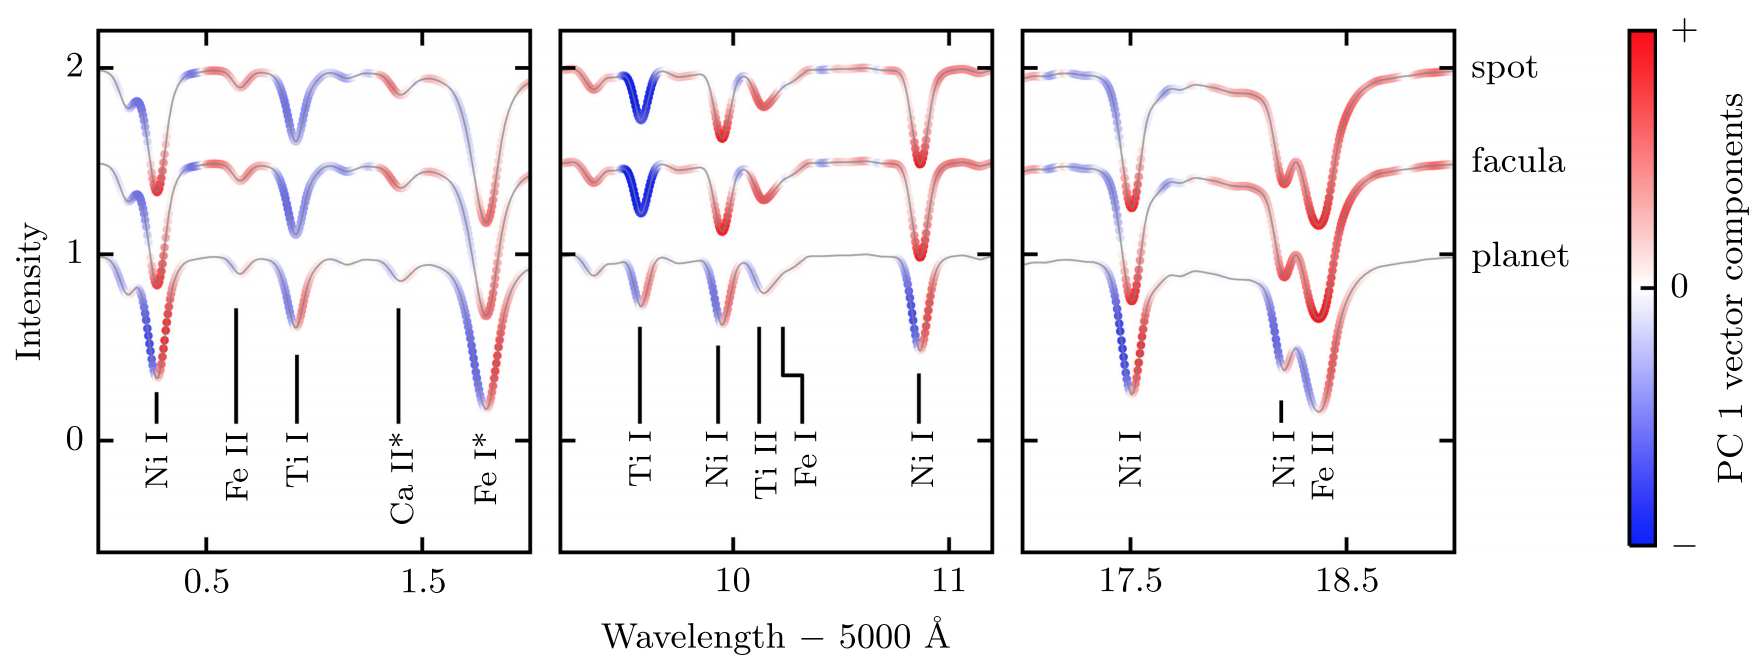
\includegraphics[width=\hsize]{figures/pca.png}
  \caption[Principal component analysis of idealized spectra containing either spots, faculae, or planets.]
          {The values of the first principal component for three spectra of a star with either an equatorial
            spot, an equatorial facula, or a circular keplerian orbit. The maximum variance (with either sign)
            in the Doppler-shifted spectrum is dominated by regions with the greatest slope and is the same
            for all spectral features. Variance in the active spectra and not equal within each line as not all
            lines respond identically to in the presence of active regions. \citep[Image credit:][]{davis17}}
  \label{fig:pca}
\end{figure}


\section{Gaussian Process Regression for Non-Parametric Activity Modelling} \label{sect:gp}
Many of the shortcomings of the activity mitigation techniques discussed in the
previous section are based on their incompleteness and their inability to
self-consistently characterize model uncertainties. For example, correlations with
activity-sensitive time series are often incomplete because the chosen indicator
is not sensitive to also activity sources present in the RVs and often result in
large RV residuals after de-correlation. Similarly, deterministic activity models
lack sensitivity to stochastic changes in activity levels due to variations in
the configuration of active regions between adjacent rotation cycles or over
significant subsets of long-term magnetic cycles. \\

Gaussian process regression models represent one such tool which aims to overcome
these shortcomings by jointly modelling planets and activity in a self-consistent
manner. This technique originally pioneered on active Sun-like stars
\citep{haywood14,rajpaul15} has been shown to reconcile disparate solutions
between observations from multiple spectrographs \citep{rajpaul17,cloutier18b},
to reconcile RV solutions for planetary systems whose favoured models are
ambiguous \citep{rajpaul17,cloutier18b}, and to disentangle neighbouring periodic
signals from planets, stellar rotation, and/or from window functions
\citep{rajpaul16,cloutier17b}.
In the following sections I will give an overview
of what Gaussian processes are and how I implement their formalism in the context
of modelling stellar activity in RV time series.

\subsection{The one dimensional Gaussian distribution}
A Gaussian process (GP) is defined as ``a collection of random variables, any
finite number of which have a joint Gaussian distribution''. In other words,
any random process\footnote{A random process is any collection of random
  variables indexed by an independent variable such as time.} for which all
finite subsets have a multivariate Gaussian distribution, is a Gaussian process.

In order to develop a visual intuition as to what this means, let us a first
consider a Gaussian random variable in one dimension. Imagine some random
process that draws a single value of a random variable $X$ in each realization of
an experiment. As an astronomer with a life
outside of astronomy, and furthermore as an astronomer who spends many of his
off-work hours being pelted with 170 gram disks of vulcanized rubber, my favourite
Gaussian random variable has to be the `goals against average' statistic:

\begin{equation}
  X = GAA \equiv \frac{\text{total number of goals against}}{\text{total number of games played}}.
\end{equation}

\noindent As a Gaussian random variable, the results of repeated experiments (i.e.
repeated draws from the empirical $GAA$ distribution for various goaltenders) can
be expressed as a probability density function of the form

\begin{equation}
  \mathcal{N}(X|\mu,\sigma) = \frac{1}{\sqrt{2\pi \sigma^2}} \exp{\left(
    -\frac{(X-\mu)^2}{2\sigma^2} \right)},
  \label{eq:gauss}
\end{equation}

\noindent which is parameterized by the mean value of $X$, $\mu$, and the variance
of $X$, $\sigma^2$. As shown in Fig.~\ref{fig:gaa1d}, the empirical distribution
of the $GAA$ for goaltenders in
the National Hockey League (NHL) over the past five seasons closely follows a
Gaussian distribution with a mean of 2.64 and a standard deviation of 0.40 goals
against per game. Hence my favourite Gaussian random variable. \\

\begin{figure}
  \centering
  %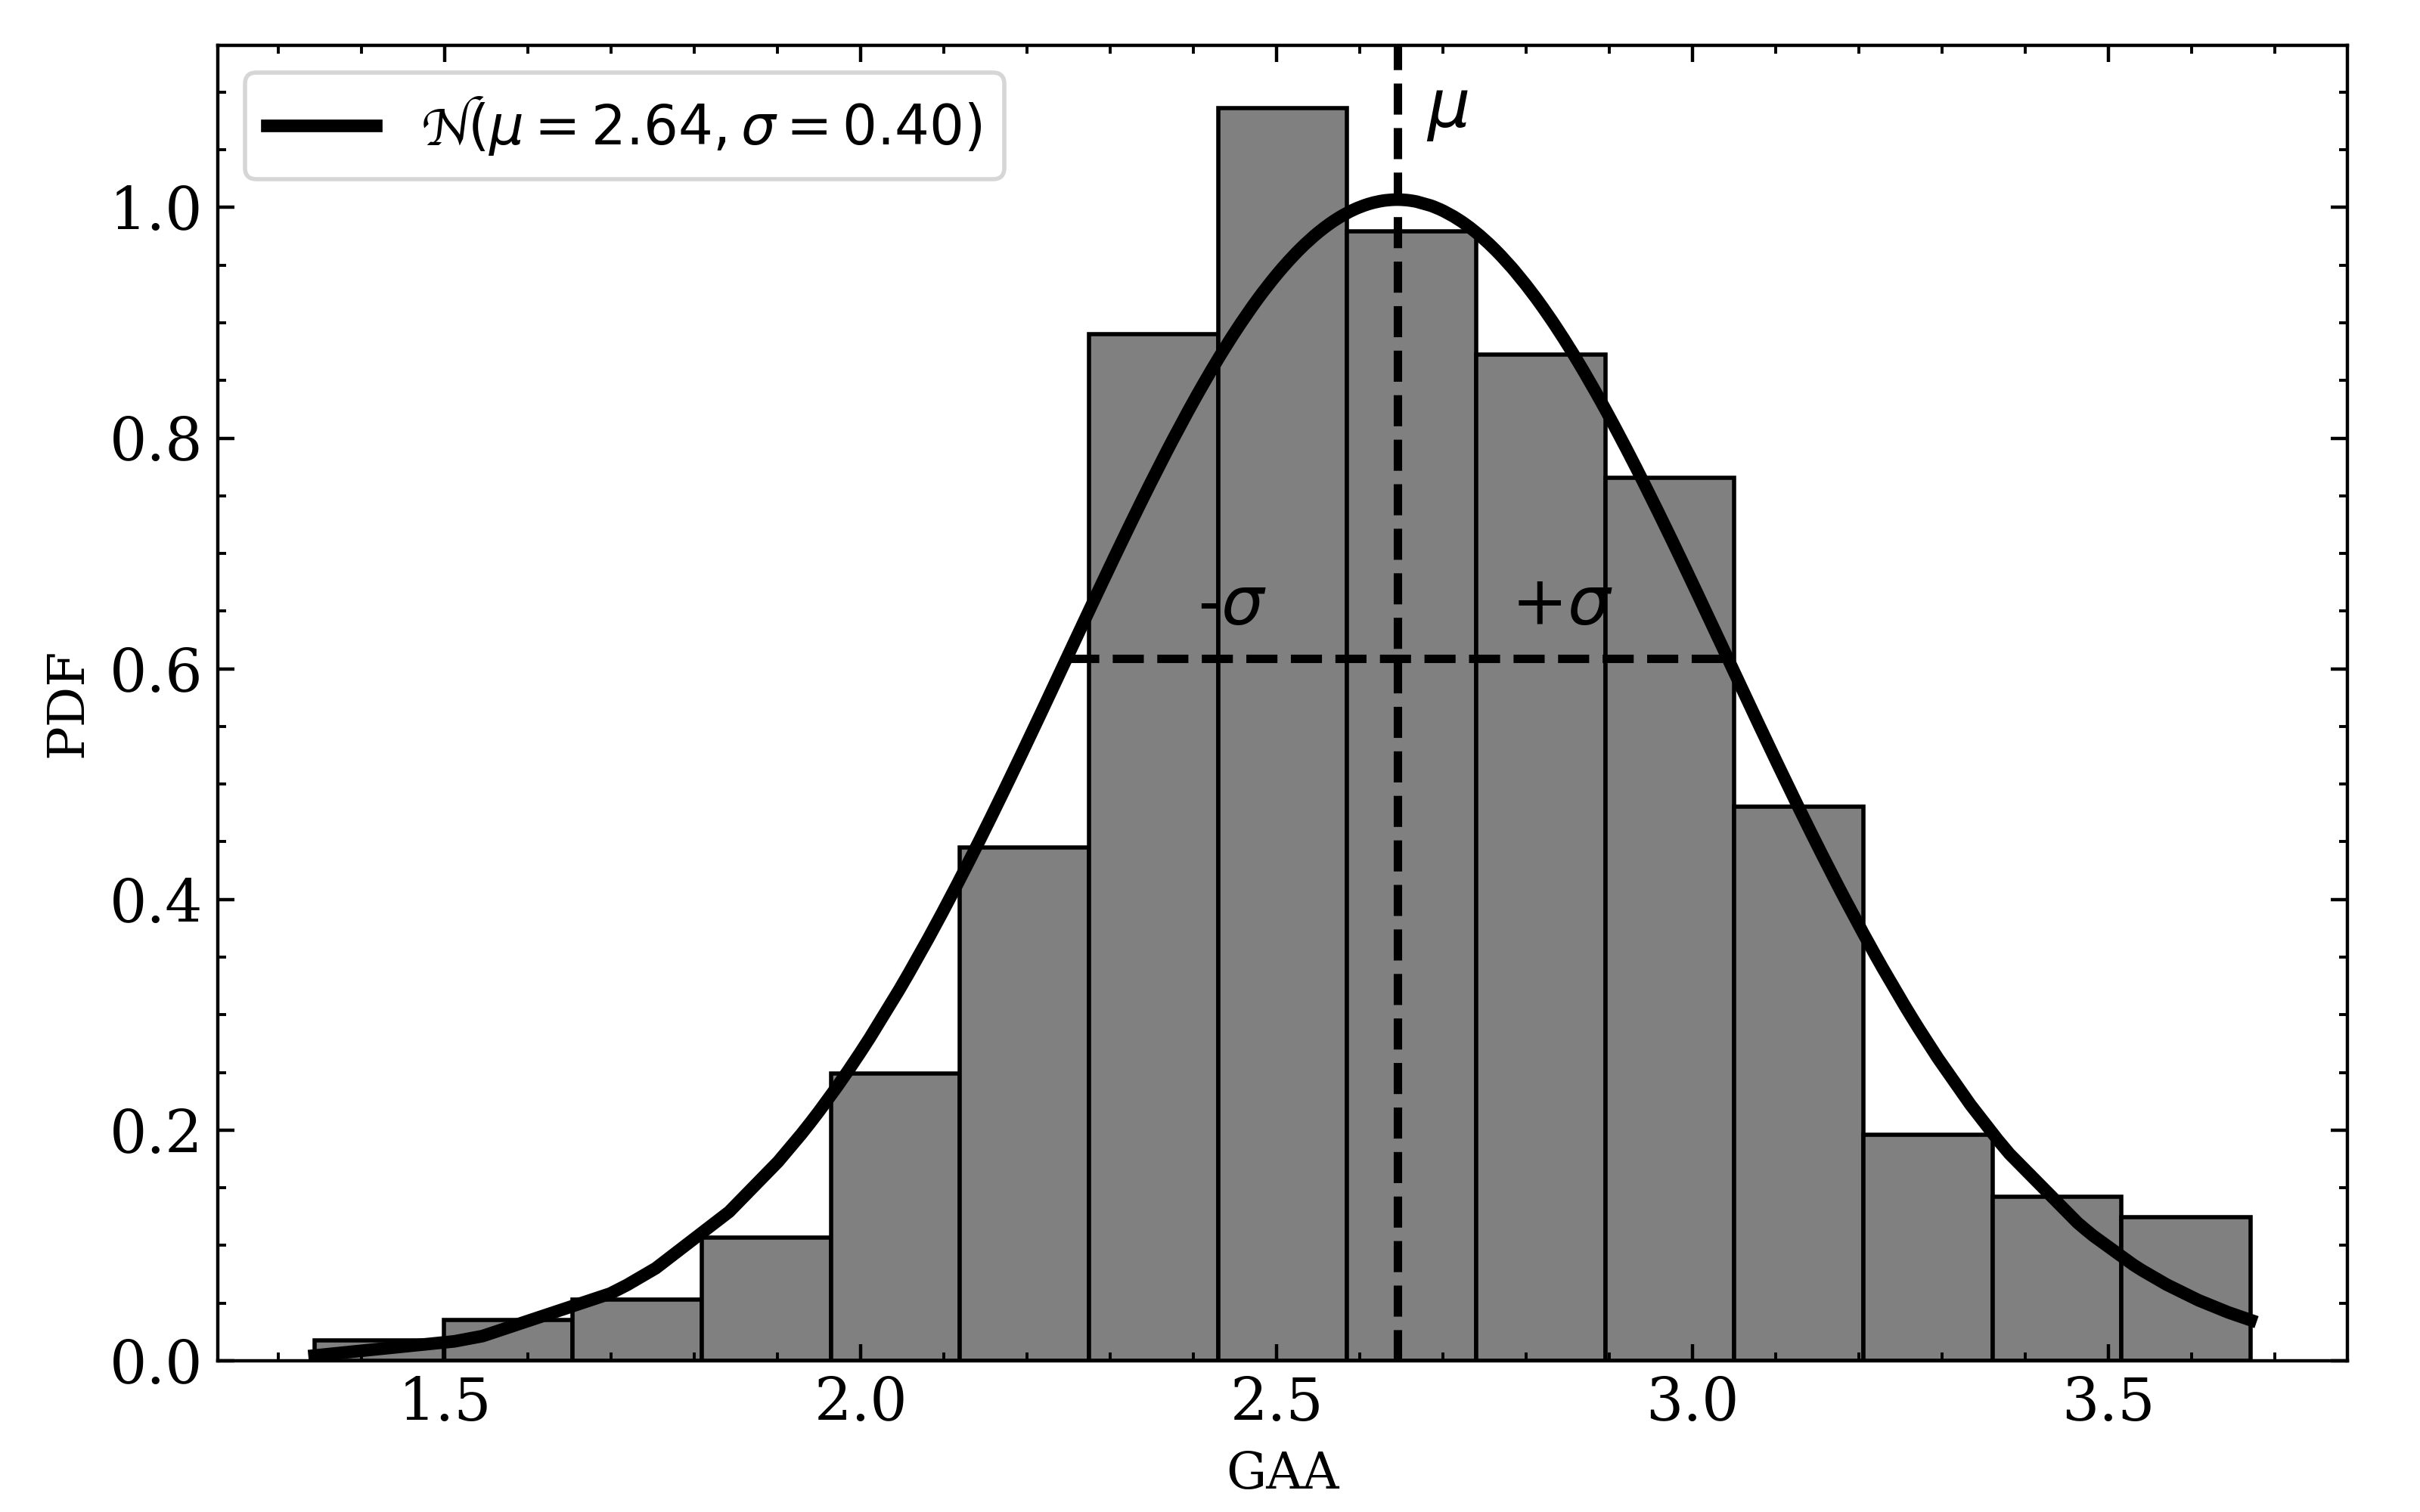
\includegraphics[width=.8\textwidth]{figures/GAA1D.png}
  \caption[Gaussian random variable in one dimension.]
      {The distribution of $GAA$ for NHL goaltenders over the past five
    seasons as an example of a Gaussian random variable. The solid line depicts
    the Gaussian probability density function with mean and standard
    deviation 2.64 and 0.40 goals against per game.}
  \label{fig:gaa1d}
\end{figure}

Before a new season begins, we can write down a prior distribution on the $GAA$
based on our prior knowledge have obtained from previous NHL seasons; i.e.
$\mathcal{N}(GAA|2.64,0.40)$. This distribution has a unique expection value and
variance describing our what we expect a given goaltender's $GAA$ to be in an
up-coming season, and as crucially, how precise that value is.

\subsection{The two dimensional Gaussian distribution}
Of course we can introduce a second Gaussian random variable and extend the 
concept of the one dimensional Gaussian distribution to two dimensions. We must
first recast the expression for the Gaussian probability density function in $k$
dimensions where $k=2$ in this scenario. Rewriting Eq.~\ref{eq:gauss} in $k$
dimensions is achieved by replacing the scalar mean and variance with a mean
$k$-vector $\boldsymbol{\mu}$ and a $k \times k$ covariance matrix $\mathbf{K}$
respectively. The updated expression for the so-called multivariate Gaussian
distribution is

\begin{equation}
  p(\mathbf{X}|\boldsymbol{\mu},\mathbf{K}) = \frac{1}{\sqrt{(2\pi)^k
      |\mathbf{K}|}} \exp{\left( -\frac{1}{2} (\mathbf{X} -
    \boldsymbol{\mu})^{\text{T}} \mathbf{K}^{-1} (\mathbf{X}-\boldsymbol{\mu})
    \right)}.
\end{equation}

\noindent The $k$-vector $\boldsymbol{\mu}$ represents the mean value of each
random variable in $\mathbf{X}=(X_1,\dots,X_k)^{\text{T}}$.
The elements of the covariance matrix
$\mathbf{K}$ represent the covariances of between each pair of random variables
with the diagonal elements representing the covariance of a random variable
with itself, or equivalently, the variance of that random variable.
The covariance between two random variables $X_1$ and $X_2$ is computed in terms
of their expected values E[$X_1$] and E[$X_2$] via

\begin{align}
  \text{cov}(X_1X_2) &= \text{E}[(X_1-\text{E}[X_1]) - (X_2-\text{E}[X_2])] \\
  &= \text{E}[X_1X_2] - \text{E}[X_1]\text{E}[X_2].
  \label{eq:coveq}
\end{align}

\noindent Note that the expected value of a Gaussian random variable is simply
its mean. \\

Consider the special case when the two Gaussian random variables under
consideration $X_1$ and $X_2$ are uncorrelated (i.e. cov$(X_1X_2)=0$). A quick
example of this is to let $X_1=GAA$ and sample $X_2$ from a Gaussian distribution
with zero mean and unit variance. The nature of sampling $X_2$ in this way ensures
that these variables are indeed uncorrelated. The corresponding covariance matrix

\begin{equation}
  \mathbf{K}(GAA,X_2) =
  \begin{bmatrix}
    0.15 & 0.00 \\
    0.00 & 0.98
  \end{bmatrix}
  \label{eq:Kuncorr}
\end{equation}

\noindent calculated using Eq.~\ref{eq:correq} is diagonal and confirms that
$X_1$ and $X_2$ are uncorrelated. This fact can be seen in the joint $X_1X_2$
distribution in Fig.~\ref{fig:uncorr2d}.
Because the variables $X_1$ and $X_2$ are uncorrelated in this example, the
measurement of a value of $X_1$ does nothing to inform us of its corresponding
$X_2$ value. That is that the prior distribution
$p(\mathbf{X}|\boldsymbol{\mu},\mathbf{K})$ is uninformative with regards to
$X_2$ when the corresponding value of $X_1$ is known. \\

\begin{figure}
  \centering
  %\includegraphics[width=.9\textwidth]{figures/uncorr_2d.png}
  \caption[Uncorrelated Gaussian random variables in two dimensions.]
      {The one and two dimensional distributions of the Gaussian random
    variables $GAA$ and draws from the standard normal disribution. The solid
    lines overlaid on their joint distribution represent the 1, 2, and 3$\sigma$
    contours. The covariance matrix (Eq.~\ref{eq:Kuncorr}) has off-diagonal
    elements equal to zero indiciating that the two variables are uncorrelated;
    a property which is largely discernable from their joint distribution.}
  \label{fig:uncorr2d}
\end{figure}

But what if we consider an alternate Gaussian random variable and set
$X_2 = SV$\% where

\begin{equation}
  X_2 = SV\% \equiv \frac{\text{total number of save made}}{\text{total number of shots faced}}
\end{equation}

\noindent is a measure of a goaltender's save percentage. In this scenario one
might expect the variables $GAA$ and $SV$\% to have some degree of correlation
as a good goaltender who boasts a low $GAA$ probably does so because of their
high $SV$\%. Indeed the covariance matrix of the $GAA$ and $SV$\% for NHL
goaltenders over the past five seasons is

\begin{equation}
  \mathbf{K}(GAA,SV\%) =
  \begin{bmatrix}
    0.1496 & -0.0037 \\
    -0.0037 & 0.0001
  \end{bmatrix}
  \label{eq:Kcorr}
\end{equation}

\noindent and has non-zero off-diagonal elements. Furthermore, the off-diagonal
elements are negative which is indicative of the anti-correlation between the
$GAA$ and the $SV$\%. This strong correlation is easily visualized in their joint
distribution in Fig.~\ref{fig:corr2d}. \\

The fact that the two variables are
correlated implies that knowledge of one variable's value provide some information
regarding the value of the second. This demonstrated in Fig.~\ref{fig:corr2d}
wherein we measure the value of the $GAA$ of the Toronto Maple Leafs goaltender
this year to be 2.57 goals per game. Not bad. Not great, but not bad. By measuring
this value we can establish a posterior distribution on Freddie's corresponding
$SV$\% given his $GAA$: $p(SV\%|GAA=2.57)$. Because the variables are dependent
on each other according to Eq.~\ref{eq:Kcorr}, this posterior distribution is
narrower (i.e. more precise) than the full $SV$\% distribution. Indeed this is
evidenced in the lower right panel of Fig.~\ref{fig:Kcorr} which compares the
two $SV$\% distributions and reveals that the dispersion in $p(SV\%|GAA=2.57)$
has approximately half of the dispersion as the full $SV$\% distribution. \\

\begin{figure}
  \centering
  %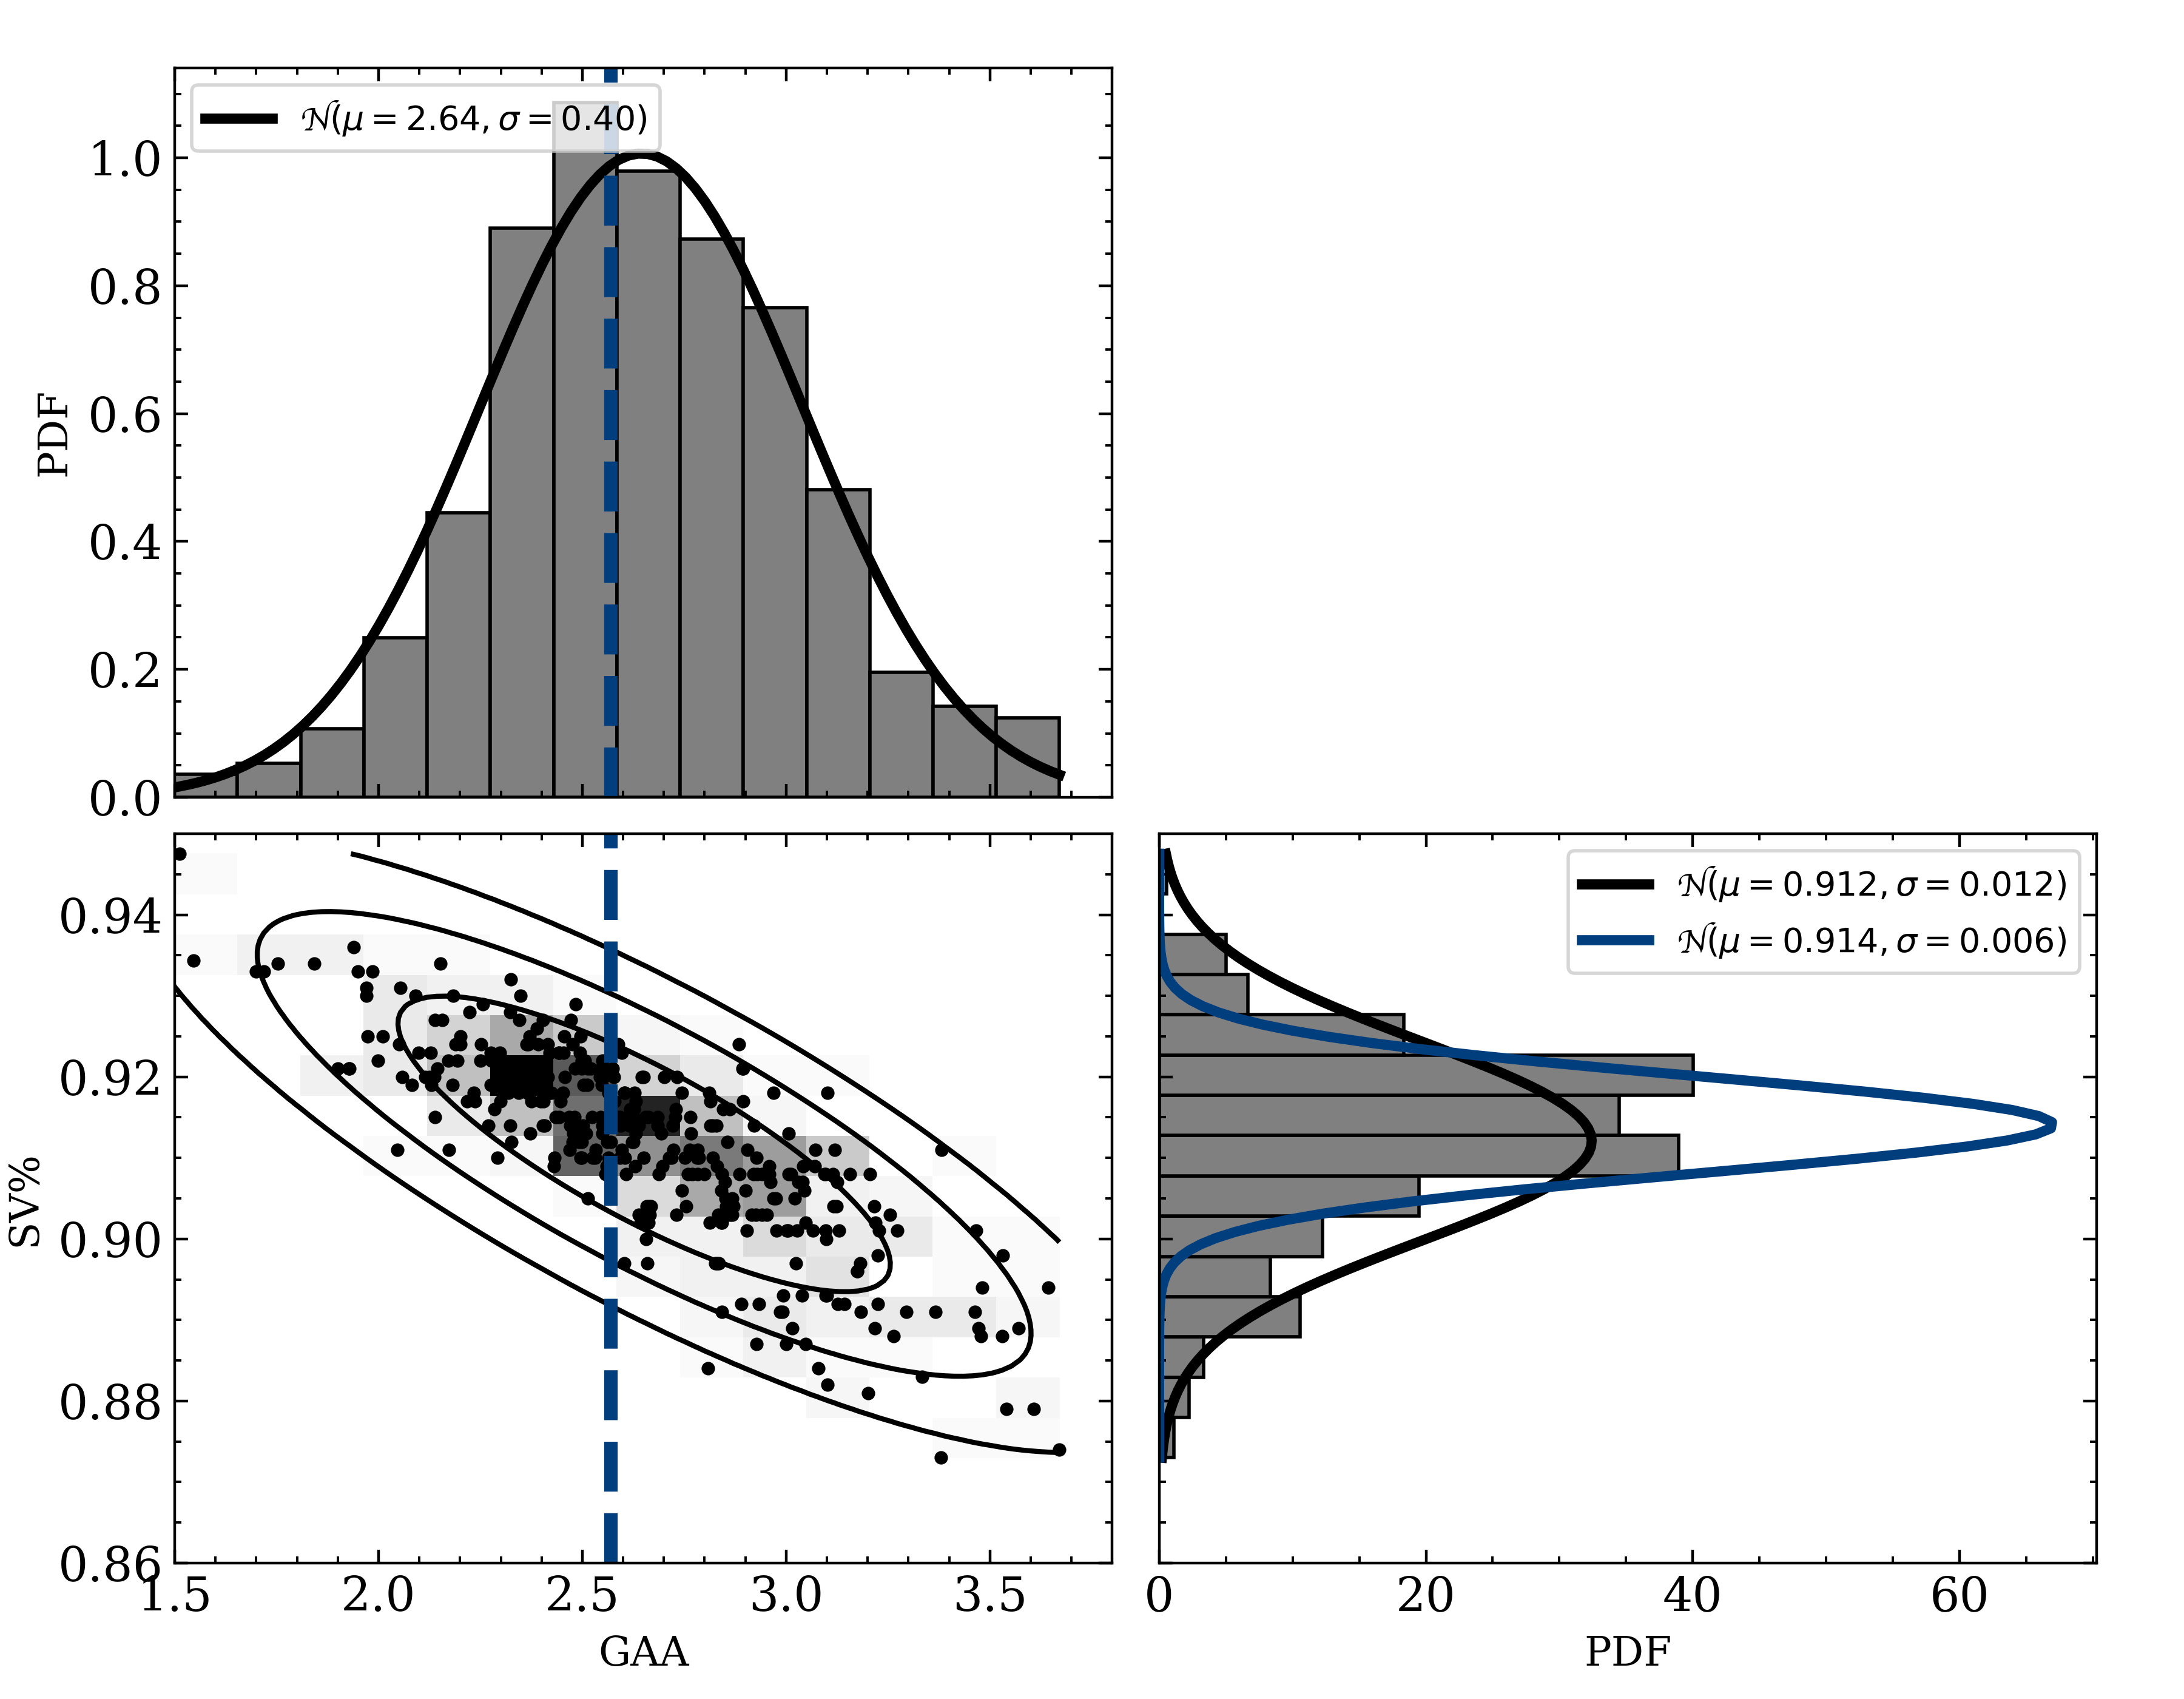
\includegraphics[width=.9\textwidth]{figures/corr_2D_HARTpost.png}
  \caption[Correlated Gaussian random variables in two dimensions.]
      {The one and two dimensional distributions of the Gaussian random
    variables $GAA$ and $SV$\%.
    The covariance matrix (Eq.~\ref{eq:Kcorr}) has negative off-diagonal
    elements describing the degree of anti-correlation between the two
    variables; a property which is largely discernable from their joint
    distribution as high values of the $SV$\% tend to correspond to a lower
    $GAA$. The correlation can be used to inform the value of $SV$\% given a
    measured value of $GAA$. This is demonstrated as the measured $GAA$ 
    for the Toronto Maple Leaf's goaltender (vertical dashed line) provides some
    additional information on the correpsonding $SV$\% whose posterior given the
    measured $GAA$ is more tightly constrained than the $SV$\% distribution for
    the entire NHL.}
  \label{fig:corr2d}
\end{figure}

The notion that the value of an unseen variable can be informed by the measurement
of another, if those variables are correlated, can have huge implications for
predictive models.


\section{Point-form Thesis: Stellar Activity Modelling in Radial Velocity
  Time Series}
\begin{itemize}
\renewcommand\labelitemi{--}
\item~\ref{sect:methods} \textbf{An Overview of Techniques for Stellar Activity
Mitigation}: hi \\
\item~\ref{sect:gp} \textbf{Gaussian Process Regression for Non-Parametric
  Activity Modelling}:
\end{itemize}
